\chapter{Spectral Method} \label{chap:spectral-method}
Spectral method is an important tool for solving problems related to partial differential equations. It can provide superior accuracy compare to other local methods such as finite difference. \cite{shen_tang_etal_spectral_2011} In this thesis, we are going to solve a polynomial eigenvalue problem, i.e. Eq.~(\ref{eq:polynomial-eigenvalue-problem}) together with specific boundary conditions.

Suppose the velocity perturbation $\tilde{v}$ can be approximated by some orthogonal basis functions $\{u_k(z)\}_{k=1}^{\infty}$ on $-1\leq z\leq 1$,
\begin{equation}
	\tilde{v} = \sum_{k=0}^{N} c_ku_k(z)
\end{equation}
where $c_k$ are coefficients to be determined. There are different choices for $u_k(z)$ including but not limited to, \cite{shen_tang_etal_spectral_2011}
\begin{itemize}
	\item $u_k(z)=T_k(z)$ (Chebyshev spectral method)
	\item $u_k(z)=L_k(z)$ (Legendre spectral method)
	\item $u_k(z)=H_k(z)$ (Hermite spectral method)
\end{itemize}
where $T_k$, $L_k$ and $H_k$ are Chebyshev, Legendre, and Hermite polynomials of degree $k$.

Using the above approximation in Eq.~(\ref{eq:polynomial-eigenvalue-problem}), and take the inner product with some other test functions $\{\psi_k(z)\}$ on $[-1,1]$, the left-hand side of Eq.~(\ref{eq:polynomial-eigenvalue-problem}) becomes a matrix equation,
\begin{equation}
	(\omega^2\mathbf{1} + \omega\mathbf{M} + \mathbf{N})\mathbf{c} = \mathbf{0}
	\label{eq:pep-matrix-equation}
\end{equation}
where $\mathbf{c} = [c_0, \cdots, c_N]^T$ is a vector of coefficients, and
\begin{equation}
	\begin{aligned}
		M_{jk} & = 2i\int_{-1}^{1}dz \; \psi_{j}\left(v_0\pdv{}{z} +\pdv{v_0}{z} \right)u_{k} \\
		N_{jk} & = \int_{-1}^{1}dz \; \psi_{j} \left[(1-v_0^2)\pdv[2]{}{z}
			-\left(3v_0 + \frac{1}{v_0}\right)\pdv{v_0}{z}\pdv{}{z}
			- \left(1-\frac{1}{v_0^2}\right)\left(\pdv{v_0}{z}\right)^2
			- \left(v_0+\frac{1}{v_0}\right)\pdv[2]{v_0}{z}\right] u_{k}
	\end{aligned}
	\label{eq:operator-matrix}
\end{equation}

Depending on the choice of the test function, spectral method can be further classified, \cite{shen_tang_etal_spectral_2011}
\begin{itemize}
	\item Galerkin: The test functions are the same as the trial ones, i.e. $\psi_k=u_k$.
	\item Collocation:  The test functions $\{\psi_k\}$ are orthogonal basis polynomials such that $\psi_k(z_j)=\delta_{jk}$, where ${z_j}$ are preassigned collocation points.
\end{itemize}

To solve Eq.~(\ref{eq:pep-matrix-equation}), we simply augment the coefficient vector to $[\mathbf{c}, \omega\mathbf{c}]^T$. Then the matrix equation can be written as an algebraic eigenvalue problem,
\begin{equation} \label{eq:eigenvalue-problem}
	\mqty[ \mathbf{0} & \mathbf{1}\\ -\mathbf{N} & -\mathbf{M} ]\mqty[ \mathbf{c}\\ \omega\mathbf{c}] = \omega\mqty[ \mathbf{c}\\ \omega\mathbf{c}]
\end{equation}
We can apply standard eigenvalue problem solver to this question to obtain the eigenvalues $\omega$ and the coefficients $\mathbf{c}$ by cutting the associated eigenvectors $[\mathbf{c}, \omega\mathbf{c}]^T$ by half.

\section{Spectral Collocation Method}
One of the methods we are going to use is called the Chebyshev collocation method. This is obtained by setting the basis functions to Chebyshev polynomials, $u_k=T_k$, and test functions satisfies $\psi_k(z_j)=\delta_{jk}$, where the collocation points are the Chebyshev points, i.e. $z_j=\cos(j\pi/N)$. By doing this, the coefficient vector $\mathbf{c}$ becomes a vector containing the values of $\tilde{v}$ at the collocation points, i.e. $\mathbf{c}=[v(z_0), \cdots, v(z_N)]^T$, and the differential operators in Eq.~(\ref{eq:operator-matrix}) become Chebyshev differentiation matrices.

\subsubsection*{Chebyshev Differentiation Matrix}
Thanks to \cite{trefethen_spectral_2000}, the construction of Chebyshev differentiation matrix is given in Fig.~\ref{fig:chebyshev-differentiation-matrix}. The Chebyshev differentiation matrix approximates the derivative of a function at the assigned Chebyshev points $\{z_j\}_{j=0}^{N}$. Suppose $\mathbf{v} = [v(z_0), \cdots, v(z_N)]^T$, then the $N$-point, $D_N$, Chebyshev differentiation matrix gives $D_N\mathbf{v} \approx [v'(z_0),\cdots, v'(z_N)]^T$. Higher order differentiation can be achieved by taking powers of $D_N$. For example, second order differentiation matrix is given by $D_N^2$.

Chebyshev differentiation matrix is basically finite difference matrix but instead of having the equal-spaced nodes, Chebyshev evaluates the derivative at Chebyshev nodes. This small change improves the accuracy dramatically. On Fig.~\ref{fig:chebyshev-vs-fd} we see that the Chebyshev achieve higher accuracy.

\begin{figure} [htbp]
	\centering
	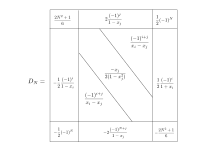
\includegraphics[width=0.7\textwidth]{figures/chebyshev-differentiation-matrix.png}
	\caption{Construction of $N$-point Chebyshev differentiation matrix. The nodes $x_j = \cos(j\pi/N)$ are Chebyshev points. Adapted from \cite{trefethen_spectral_2000}.}
	\label{fig:chebyshev-differentiation-matrix}
\end{figure}

\begin{figure}
	\centering
	\includegraphics[width=0.7\textwidth]{figures/chebyshev-vs-fd.png}
	\caption{Comparison of accuracy between Chebyshev differentiation matrix and 2nd order finite difference differentiation matrix. Both methods are applied to compute the derivative of function $f(x)=\ln(2+\sin(x))$ on $[-1,1]$. Chebyshev differentiation achieve higher accuracy and converge faster than finite difference.}
	\label{fig:chebyshev-vs-fd}
\end{figure}

\subsubsection*{Dirichlet Boundary}
To implement Dirichlet boundary condition, there is no need to modify anything. In practice, for a $(N+1)\times(N+1)$ Chebyshev differentiation matrix $D_N$, we only take its interior $N\times N$ by stripping the first and last columns and rows. See Fig.~\ref{fig:interior-of-chebyshev-differentiation-matrix}. Same procedure applies to higher order differentiation.

\begin{figure} [htpb]
	\centering
	\includegraphics[width=0.7\textwidth]{figures/interior-of-chebyshev-differentiation-matrix.png}
	\caption{Since the function $v$ is zero at $x_0$ and  $x_N$, the first and last columns has no effect and the same argument applies to first and last rows. Adapted from \cite{trefethen_spectral_2000}.}
	\label{fig:interior-of-chebyshev-differentiation-matrix}
\end{figure}

Listing.~\ref{code:spectral-collocation-dirichlet} has the pseudocode for solving Eq.~(\ref{eq:pep-matrix-equation}).

\begin{lstlisting}[language=Python, float, floatplacement=H, caption={Pseudocode for solving polynomial eigenvalue problem with Dirichlet boundary condition.}, label=code:spectral-collocation-dirichlet]
import numpy as np
x, D1, D2 = Chebyshev(N)	
A11 = np.zeros_like(D1)
A12 = np.eye(*D1.shape)
A21 = -np.diag(1-v0**2)@D2 \
        + np.diag((3*v0 + 1/v0)*(D1@v0))@D1 \
        + np.diag((1-1/v0**2)*(D1@v0)**2) \
        + np.diag((v0+1/v0)*(D2@v0)) 
A22 = -2j*(np.diag(v0)@D1 + np.diag(D1@v0))
A = np.block([[A11[1:-1,1:-1], A12[1:-1,1:-1]],
              [A21[1:-1,1:-1], A22[1:-1,1:-1]]])
omega, V = np.linalg.eig(A)
# pad the two ends by 0 (dirichlet boundary)
V = np.pad(V,((1,1),(0,0)))
\end{lstlisting}

\subsubsection*{Fixed-Open Boundary}
To implement fixed-open boundary condition, i.e. $\tilde{v}(-1)=\tilde{v}'(1)=0$. Notice that $\tilde{v}'(-1)$ can be expressed as,
\begin{equation}
	0 = \tilde{v}'(1) = \sum_{j=0}^{N}D_{ij}\tilde{v}_j
\end{equation}
where $\tilde{v}_j=\tilde{v}(z_j)$ is the evaluation of $\tilde{v}$ at Chebyshev points $z_j=\cos(j\pi/N)$. By rearranging the terms, we get the expression of $\tilde{v}_0$ in terms of $\tilde{v}$ at other collocation points.
\begin{equation}
	\tilde{v}_0 = -\frac{1}{D_{00}}\sum_{j=1}^{N} D_{0j}\tilde{v}_j
	\label{eq:expression-for-first-value}
\end{equation}
To incorporate this information into the differentiation matrix, we modify the expressions for evaluating the derivatives at point $x_1$,
\begin{align}
	\tilde{v}'_{1}  & = \sum_{j=0}^{N}D_{1j}\tilde{v}_j = \sum_{j=1}^{N}\left(D_{1j} - \frac{D_{10}}{D_{00}}D_{0j}\right)\tilde{v}_j       \\
	\tilde{v}''_{1} & = \sum_{j=0}^{N}D^2_{1j}\tilde{v}_j = \sum_{j=1}^{N}\left(D^2_{1j} - \frac{D^2_{10}}{D_{00}}D_{0j}\right)\tilde{v}_j
\end{align}
This indicates the new differentiation matrices should be
\begin{align}
	D'_{ij} = \begin{cases}
		          D_{ij}, \quad                               & \text{if $i\neq 1$} \\
		          D_{1j} - \frac{D_{10}}{D_{00}}D_{0j}, \quad & \text{if $i=1$}
	          \end{cases} \\
	D'^2_{ij} = \begin{cases}
		            D^2_{ij}, \quad                                 & \text{if $i\neq 1$} \\
		            D^2_{1j} - \frac{D^2_{10}}{D_{00}}D_{0j}, \quad & \text{if $i=1$}
	            \end{cases}
\end{align}
After getting the eigenfunctions $\mathbf{c} = [\tilde{v}_1, \cdots, \tilde{v}_N]^T$, we need to prepend $\tilde{v}_0$ to $\mathbf{c}$ using Eq.~(\ref{eq:expression-for-first-value}). See Listing.~\ref{code:spectral-collocation-fixed-open} for pseudocode.


\begin{lstlisting}[language=Python, float, floatplacement=H, caption={Pseudocode for solving polynomial eigenvalue problem with fixed-open boundary condition.}, label=code:spectral-collocation-fixed-open]
import numpy as np
x, D1, D2 = Chebyshev(N)	
D1v = D1
D2v = D2
D1v[1,:] = D1[1,:] - D1[1,0]/D1[0,0]*D1[0,:]
D2v[1,:] = D2[1,:] - D2[1,0]/D1[0,0]*D1[0,:]

A11 = np.zeros_like(D1)
A12 = np.eye(*D1.shape)
A21 = -np.diag(1-v0**2)@D2v \
        + np.diag((3*v0 + 1/v0)*(D1@v0))@D1v \
        + np.diag((1-1/v0**2)*(D1@v0)**2) \
        + np.diag((v0+1/v0)*(D2@v0))
A22 = -2j*(np.diag(v0)@D1v + np.diag(D1@v0))

A = np.block([[A11[:-1,:-1], A12[:-1,:-1]],
              [A21[:-1,:-1], A22[:-1,:-1]]])
omega, V = np.linalg.eig(A)
# pad 0 to the last row then modify them
V = np.pad(V,((1,0),(0,0)))
for j in range(V.shape[1]):
    V[0,j] = -(D1[0,1:]@V[1:,j])/D1[0,0]
\end{lstlisting}


\section{Spectral Galerkin Method}
Another spectral method we used in the numerical experiments is the Legendre-Galerkin method. Meaning that the basis functions are chosen to be the compact combinations of Legendre polynomials, \cite{shen_tang_etal_spectral_2011}
\begin{equation}
	u_k(z) = L_k(z) + a_kL_{k+1}(z) + b_kL_{k+2}(z)
\end{equation}
where the parameters $\{a_k,b_k\}$ are chosen to satisfy the boundary conditions. The test functions are the same as the basis functions.

\subsubsection*{Dirichlet Boundary}
The necessary parameters to make $u_k(\pm 1) = 0$ are $a_k=0, b_k=-1$. The basis functions are therefore,
\begin{equation}
	u_k(z) = L_k(z) - L_{k+2}(z)
\end{equation}

\subsubsection*{Fixed-Open Boundary}
The necessary parameters to make $u_k'(\pm 1) = 0$ are $a_k=(2k+3)/(k+2)^2, b_k=-(k+1)^2/(k+2)^2$. The basis functions are therefore,
\begin{equation}
	u_k(z) = L_k(z) + \frac{2k+3}{(k+2)^2}L_{k+1}(z) - \frac{(k+1)^2}{(k+2)^2}L_{k+2}(z)
\end{equation}

The spatial derivatives in Eq.~(\ref{eq:operator-matrix}) should utilize the Chebyshev differentiation matrix, it ensures better accuracy.


\section{Spectral Theory in Finite-Dimensional Normed Spaces}
Spectral method transforms the polynomial eigenvalue problem to an algebraic eigenvalue problem. For completion, some important linear algebra results are included in this section.

Let $X$ be a finite dimensional normed space and $\hat{T}: X \to X$ a linear operator. Since any linear operator can be represented by a matrix, the spectral theory of $\hat{T}$ is essentially matrix eigenvalue theory. \cite{kreyszig_introductory_1978} Let $A$ be a matrix representation of $\hat{T}$, then we have the definition.

\begin{definition} [Kryszig \cite{kreyszig_introductory_1978}]
	An eigenvalue of a square matrix $A$ is a complex number $\lambda$ such that
	\[ Ax = \lambda x \]
	has a solution $x\neq 0$.This $x$ is called an \textbf{eigenvector} of $A$ corresponding to that eigenvalue $\lambda$.The set $\sigma(A)$ of all eigenvalues of $A$ is called the \textbf{spectrum} of $A$. Its complement $\rho(A) = \mathbb{C}-\sigma(A)$ in the complex plane is called the \textbf{resolvent} set of $A$.
\end{definition}

By choosing different bases in $X$, we can have different matrix representation of $\hat{T}$. We need to make sure the eigenvalues of a linear operator is independent of the basis chosen. Fortunately, a theorem ensures that.

\begin{theorem} [Kryszig \cite{kreyszig_introductory_1978}]
	All matrices representing a given linear operator $\hat{T}: X \to X$ on a finite dimensional normed space $X$ relative to various bases for $X$ have the same eigenvalues.
\end{theorem}


Moreover, we don't need to worry about the existence of eigenvalues of a linear operator. The following theorem shows the existence of them.
\begin{theorem} [Kryszig \cite{kreyszig_introductory_1978}]
	A linear operator on a finite dimensional complex normed space $X\neq{O}$ has at least one eigenvalue.
\end{theorem}

\section{Spectral Pollution and Spurious Modes}
In this section, we will discuss an important phenomenon we observe throughout the numerical experiments using spectral method. It is the phenomenon of spectral pollution. Then we will provide a method to filter these spurious modes.

Spectral pollution refers to the phenomenon which some eigenvalues are not converging to the correct value when the mesh density is increased. The wrong eigenvalues are referred as spurious modes. When solving eigenvalue problems using spectral methods with finite difference or finite element approximations, spectral pollution might occur. \cite{llobet_spectral_1990} The cause of the spectral pollution is originated from the improper discretization of the differential operators. In the following sections, we are going to take a closer look at the differential operators in finite difference method, and reveal the occurrence of spurious modes when solving Eq.~(\ref{eq:constant-v-problem-dirichlet}).

\subsection{Analysis of Numerical Spectrum}
In this section, we will analyze the analytical and numerical dispersion relation of Eq.~(\ref{eq:constant-v-problem-dirichlet}). It is a special case, i.e. $v_0=$constant, of a more general problem Eq.~(\ref{eq:polynomial-eigenvalue-problem}). The analytical dispersion relation can be obtained by substituting $\tilde{v} = \exp(-i\omega t + kx)$ into Eq.~(\ref{eq:constant-v-problem-dirichlet}),
\begin{equation} \label{dispersion-relation}
	\omega = k(v_0 \pm 1)
\end{equation}
The dispersion relation suggests that the eigenvalue $\omega$ should be real.

Now let's analyze the dispersion relation produced by finite difference. To do this we need to first understand the effect of the differential operators on function $\tilde{v}$ in finite difference. If we assume $\tilde{v}\sim \exp(ikx)$, and let $\beta\equiv kh/2$. Then in finite difference discretization scheme, the differential operators $\dv*[n]{z}$ are equivalent to the following factors \cite{llobet_spectral_1990},
\begin{equation}
	\begin{aligned}
		\dv[0]{z} \quad \to \quad & G_0 = 1                                                              \\
		\dv[1]{z} \quad \to \quad & G_1 = [\exp(2i\beta)-\exp(-2i\beta)]/2h = (i/h)\sin(2\beta)          \\
		\dv[2]{z} \quad \to \quad & G_2 = [\exp(2i\beta)-2-\exp(-2i\beta)]/h^2 = (2/h^2)(\cos(2\beta)-1)
	\end{aligned}
	\label{eq:G-operator}
\end{equation}

Using the G-operators, Eq.~(\ref{eq:G-operator}), the discretized equation of Eq.~(\ref{eq:constant-v-problem-dirichlet}) becomes
\begin{equation} \label{eq:discretized-eq-G}
	(\omega^2G_0 + \omega G_1 + G_2)\tilde{v} = 0
\end{equation}

Solving Eq.~(\ref{eq:discretized-eq-G}), we obtain the numerical dispersion relation,
\begin{equation} \label{dispersion-relation-G}
	\omega = \frac{2\sin(\beta)}{h}\left(v_0 \pm \sqrt{1 - v_0^2\sin[2](\beta)}\right)
\end{equation}

Given $h$ (fixed the mesh resolution), we see that
\begin{itemize}
	\item $\omega$ is real for all $k$ if $v_0 < 1$.
	\item $\omega$ is complex for large $k$, more specifically $k>h/2\arcsin(1/v_0)$, if $v_0 > 1$.
	\item For small $k$, meaning $k\to 0$, Eq.~(\ref{dispersion-relation-G}) is a good representation for the analytical dispersion relation, Eq.~(\ref{dispersion-relation}).
\end{itemize}

\begin{figure}[H]
	\centering
	\begin{subfigure}[b]{0.5\linewidth}
		\includegraphics[width=\linewidth]{figures/eigvals-bad}
		\caption{Bad eigenvalues}
	\end{subfigure}%
	\begin{subfigure}[b]{0.5\linewidth}
		\includegraphics[width=\linewidth]{figures/eigvecs-bad}
		\caption{Bad eigenfunctions}
	\end{subfigure}
	\caption{Spurious modes.}
	\label{fig:results-bad}
\end{figure}

One way to filter the spurious modes is to remove all modes with $k>h/2 \arcsin(1/v_0)$, see Fig.~\ref{fig:results-filter-k}. However, this is not a good way to deal with general cases because it requires the solution to the discretized problem Eq.~(\ref{eq:discretized-eq-G}). For general problem with non-constant velocity profile, it is hard to solve the discretized problem directly.

\begin{figure}[H]
	\centering
	\begin{subfigure}[b]{0.5\linewidth}
		\includegraphics[width=\linewidth]{figures/eigvals-good}
		\caption{Good eigenvalues}
	\end{subfigure}%
	\begin{subfigure}[b]{0.5\linewidth}
		\includegraphics[width=\linewidth]{figures/eigvecs-good}
		\caption{Good eigenfunctions}
	\end{subfigure}
	\caption{Filter out the spurious modes with $k>h/2\arcsin(1/v_0)$.}
	\label{fig:results-filter-k}
\end{figure}

\subsection{Convergence Test}
A better way to filter the spurious modes is by doing a "convergence test". Since the frequency Eq.~(\ref{dispersion-relation-G}) is changing with mesh resolution $h$. From Fig.~\ref{fig:convergence-test} we see that only the true eigenmodes converge while the eigenvalues of spurious eigenmodes changes dramatically under different resolutions. By simply solving the discretized problem using spectral method under different mesh resolution, we can pick up the true eigenmodes by observing their convergence, and filter out the spurious eigenmodes which change dramatically.

\begin{figure} [htbp]
	\centering
	\includegraphics[width=\textwidth]{figures/eigenvalues-eigenfunctions-convergence.png}
	\caption{The figure shows eigenvalues under different resolutions. (a)
		Weird-shape eigenfunctions are associated with spurious eigenvalues. (b) Good
		eigenfunctions are associated with true eigenvalues. (c) True eigenvalues are
		roughly at the same location under different resolutions.}
	\label{fig:convergence-test}
\end{figure}